% arara: clean: {extensions: ['log','out','snm','blg','bbl','nav','aux','toc']}
% arara: lualatex
% arara: bibtex
% arara: lualatex
% arara: lualatex
% arara: clean: {extensions: ['log','out','snm','blg','bbl','nav','aux','toc']}

\def\footer#1{\def\insertfooter{#1}}
%--------------------------------------------------------------------------------------
%	PACKAGES AND OTHER DOCUMENT CONFIGURATIONS
%--------------------------------------------------------------------------------------
\documentclass[final]{beamer}

\usepackage[scale=1.150]{beamerposter} % Use the beamerposter package
\usetheme{MUWposter} % Use the MUWposter theme supplied with this template
% Include a logo of your project if desired
\logo{\pgfputat{\pgfxy(-11,107)}{\pgfbox[center,base]{
\includegraphics[width=8cm]{ABETlogo.png}}}}
\usepackage{multicol}
\usepackage{array}
%The following two are column definitions for the aknowledgements section
\newcolumntype{L}{>{\arraybackslash}m{22cm}}
\newcolumntype{S}{>{\arraybackslash}m{5cm}}
\usepackage{pgf}  
\usepackage{mathtools}
\usepackage{amsmath,amsthm,amssymb}
\usepackage{exscale}
\usepackage{ushort}
\usepackage{setspace}
\usepackage[square,numbers]{natbib}
\usepackage{url}
\bibliographystyle{abbrvnat}
\renewcommand{\vec}[1]{\ushort{#1}}
\renewcommand{\vec}[1]{\mathbf{#1}}
\definecolor{greenMUW}{RGB}{60,191,174}
\definecolor{blueMUW}{RGB}{17,29,79}
\definecolor{skinMUW}{RGB}{254,228,217}
\definecolor{hellblauMUW}{RGB}{95,180,229}
%-----------------------------------------------
%  START Set the colors
%  Uncomment to apply colors you want to use.
%-----------------------------------------------
\colorlet{themecolor}{jblue}%unibeige!50!black
\usebackgroundtemplate{
\includegraphics{UNI_skin.pdf}}

%\colorlet{themecolor}{skinMUW}
%\colorlet{themecolor}{blueMUW}
%\usebackgroundtemplate{
\includegraphics{MUW_skin.pdf}}

%%\colorlet{themecolor}{blueMUW}
%\colorlet{themecolor}{hellblauMUW}
%\usebackgroundtemplate{
\includegraphics{MUW_hellblau.pdf}}
%-----------------------------------------------
%  END Set the colors
%-----------------------------------------------

%-----------------------------------------------
%  START Set the width of the columns
%-----------------------------------------------
\setlength{\paperwidth}{33.1in} % A0 width: 46.8in
\setlength{\paperheight}{46.8in} % A0 height: 33.1in
\newlength{\sepmargin}
\newlength{\sepwid}
\newlength{\onecolwid}
\newlength{\twocolwid}
\newlength{\threecolwid}

% The following measures are used for 2 columns
\setlength{\sepmargin}{0.055\paperwidth} % Separation width (white space) between columns
\setlength{\sepwid}{0.03\paperwidth} % Separation width (white space) between columns
\setlength{\onecolwid}{0.43\paperwidth} % Width of one column
\setlength{\twocolwid}{0.9\paperwidth} % Width of two columns

%-----------------------------------------------------------
% The following measures are used for 3 columns
%\setlength{\sepmargin}{0.06\paperwidth} % Separation width (white space) between columns
%\setlength{\sepwid}{0.02\paperwidth} % Separation width (white space) between columns
%\setlength{\onecolwid}{0.28\paperwidth} % Width of one column
%\setlength{\twocolwid}{0.58\paperwidth} % Width of two columns
%\setlength{\threecolwid}{0.88\paperwidth} % Width of three columns
%\setlength{\columnsep}{30pt}

%-----------------------------------------------
%  END Set the width of the columns
%-----------------------------------------------

%--------------------------------------------------------------------------------------
%	TITLE SECTION 
%--------------------------------------------------------------------------------------
\setbeamertemplate{title}[left]
\setbeamertemplate{frametitle}[default][left]
%\setmainfont{Georgia}

\title{Un algoritmo aleatorizado para calcular la mediana} % Poster title

\author[shortname]{E. Talla Chumpitáz\inst{1}, C. Aznarán Laos\inst{2}, M. Silva Menejes\inst{2} y J. Jáuregui Alvarado\inst{2}.}
\institute[shortinst]{\inst{1}Escuela Profesional de Ciencia de la Computación, Universidad Nacional de Ingeniería, Perú.\and
\inst{2}Escuela Profesional de Matemática, Universidad Nacional de Ingeniería, Perú.
}
%\institute{Klinik, Medizinische Universität Wien, Schriftgröße variabel} % Institution(s)
%--------------------------------------------------------------------------------------
\newcommand{\MVAt}{{\usefont{U}{mvs}{m}{n}\symbol{`@}}}
\renewcommand{\figurename}{Figura}
\begin{document}

\addtobeamertemplate{block end}{}{\vspace*{1ex}} % White space under blocks
\addtobeamertemplate{block alerted end}{}{\vspace*{0ex}} % White space under highlighted (alert) blocks
\setlength{\belowcaptionskip}{2ex} % White space under figures
\setlength\belowdisplayshortskip{1ex} % White space under equations

\begin{frame}[t] % The whole poster is enclosed in one beamer frame

	\begin{columns}[t] % The whole poster consists of two major columns

		\begin{column}{\sepmargin}\end{column}

		\begin{column}{\onecolwid} % The first column

			\begin{block}{Objetivos}
				El objetivo de este trabajo es comparar los diferentes algoritmos de ordenación con respecto al tiempo de ejecución medio que tarda en calcular la mediana de una data.
			\end{block}

			\vspace{-0.5cm}

			\begin{block}{Introducción}
				En el mundo de la estadística existen distintas \emph{medidas de tendencia central}, entre las más comunes se encuentran la \emph{media}, la \emph{mediana} y la \emph{moda}, en este reporte nos enfocaremos en la \emph{mediana}, repasando desde su origen, su importancia y sus aplicaciones prácticas mediante un ejemplo con datos estadísticos.
			\end{block}

			\begin{block}{Metodología}% o parte experimental
			Para hallar la mediana de un conjunto de datos, se debe de utilizar un algoritmo de \emph{ordenamiento} y de \emph{búsqueda}, ya que no se sabe si el conjunto de datos está ordenado. Para ello se analiza primero los algoritmos de \emph{búsqueda}.\\[\baselineskip]
			Aplicado a nuestro objetivo sería ineficiente buscar secuencialmente la \emph{mediana}, ya que no necesitamos recorrer toda la cadena para hallarlo, aún peor cuando no está ordenado.
			\end{block}

			\vspace{-0.5cm}

			\begin{block}{Conclusiones}
				\begin{itemize}
					\item La aleatorización del arreglo ayudó al algoritmo \emph{quick select} a tener una complejidad $\mathcal{O}(n)$.

					\item En el lenguaje de programación R, el algoritmo más eficiente es \emph{Radix}, pero implementado en el lenguaje de programación C, el algoritmo más eficiente es \emph{Random Selection}.
				\end{itemize}
			\end{block}

			\begin{block}{Referencias bibliográficas}
				\vspace{-0.5cm}
				\nocite{*} % Insert publications even if they are not cited in the poster
				\bibliography{bibliog.bib}
			\end{block}

			\begin{block}{\large Agradecimientos}
				Van a faltar palabras para agradecer a las personas que se han involucrado en la realización de este trabajo, sin embargo, el profesor Cesar Lara Ávila merece un reconocimiento especial ya que gracias a sus consejos y correcciones hoy pudimos culminar este trabajo.
      \end{block}

			\begin{alertblock}{\large Información del contacto}
			\vspace*{-0.5cm}
      	\begin{footnotesize}
					\begin{itemize}
						\item Autor principal: \href{mailto:erwinleo_98@hotmail.com}{erwinleo\textunderscore 98\MVAt hotmail.com}
						\item Autor secundario: \href{mailto:caznaranl@uni.pe}{caznaranl\MVAt uni.pe}
						\item Autor secundario: \href{mailto:miller_silva_96@hotmail.com}{miller\textunderscore silva\textunderscore 96\MVAt hotmail.com}
						\item Autor secundario: \href{mailto:jjaureguia@uni.pe}{jjaureguia\MVAt uni.pe}
						\item Profesor investigador: \href{mailto:cesarlaraavila@gmail.com}{cesarlaraavila\MVAt gmail.com}
						\item Link del repositorio: \href{https://github.com/carlosal1015/A-randomized-algorithm-to-calculate-the-median}{github.com/carlosal1015/A-randomized-algorithm-to-calculate-the-median}
					\end{itemize}
				\end{footnotesize}
			\end{alertblock}
		\end{column}

		\begin{column}{\sepwid}\end{column}

		\begin{column}{\onecolwid} %The second column

			\begin{block}{Resumen}
				En el ámbito de la estadística y probabilidad existe una controversia sobre cuándo emplear la \emph{mediana} como medida de tendencia central. El objetivo de este artículo es valorar mediante un programa en R su utilidad. Para poder llevar a cabo esta investigación, se han revisado artículos científicos similares y consultado la base de datos de World Bank Open Data, ScienceDirect y otros de donde se extrajo la muestra para la experimentación.\\[0.5\baselineskip]
				Después de haber probado diferentes métodos para el cálculo aleatorizado de la mediana, llamamos ``random quicksort'' a nuestro programa más eficiente.
			\end{block}
			\vspace{-0.5cm}

			\begin{block}{Resultados y discusiones}
				La mediana es un estadístico robusto que incluso aunque los extremos de los datos se vean alterados, la mediana permanece invariable muy útil cuando se trabaja con distribuciones sesgadas.\\[0.5\baselineskip]
				Cuando se hacen las comparaciones, el programa implementado en el lenguaje C, el \emph{random quick select} es más rápido que el algoritmo de ordenación \emph{Radix}, pero cuando se implementa en el lenguaje R, \emph{Radix} obtiene la complejidad $\mathcal{O}(1)$, es decir, ya no depende del tamaño de datos $n$.
			\end{block}
			\vspace{-0.8cm}

			\begin{figure}
				\centering
				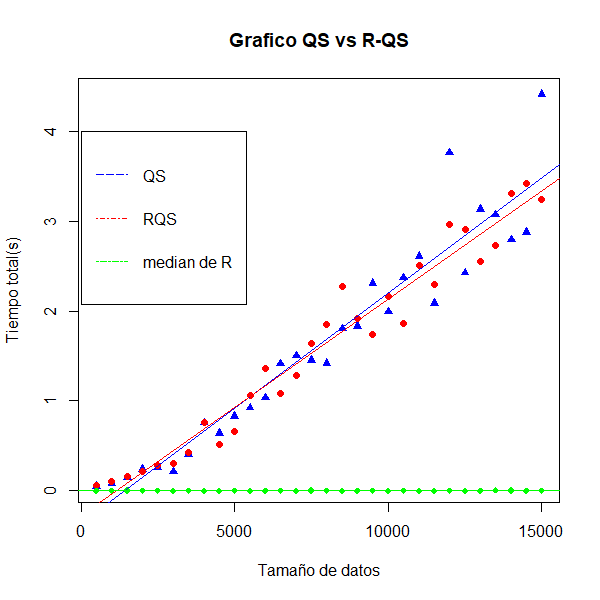
\includegraphics[width=.73\linewidth]{Rplot.png}
				\caption{Gráfico Quick sort vs Random Quick sort programado en R.}
			\end{figure}
			\vspace{-1.5cm}
			\begin{figure}
				\centering
				\includegraphics[width=.73\linewidth]{Cplot.png}
				\caption{Gráfico Quick sort vs Random Quick sort programado en C.}
			\end{figure}
			\vspace{-0.9cm}
		\end{column}

		\begin{column}{\sepmargin} \end{column}
	\end{columns} 

	\begin{columns}[t] % Split up the two columns wide column again

		\begin{column}{\sepmargin} \end{column}
		\begin{column}{\onecolwid} % The first column
		\end{column} % End of the first column

		\begin{column}{\sepwid}\end{column} % Empty spacer column
		\begin{column}{\onecolwid} % Begin a column 
		\end{column}% End of the second column

		\begin{column}{\sepmargin}\end{column} % Empty spacer column

	\end{columns} % End of all the columns in the poster

\end{frame} % End of the enclosing frame

\end{document}